% *********************************************************************
% © 2021–2026 Jeremy Sylvestre
%
% Permission is granted to copy, distribute and/or modify this document
% under the terms of the GNU Free Documentation License, Version 1.3 or
% any later version published by the Free Software Foundation; with no
% Invariant Sections, no Front-Cover Texts, and no Back-Cover Texts. A
% copy of the license is included in the appendix entitled “GNU Free
% Documentation License” that appears in the output document of this
% PreTeXt source code. All trademarks™ are the registered® marks of
% their respective owners.
%
% *********************************************************************

\newcommand*{\xmin}{-0.5}
\newcommand*{\xmax}{5.5}
\newcommand*{\ymin}{-2.5}
\newcommand*{\ymax}{2.5}

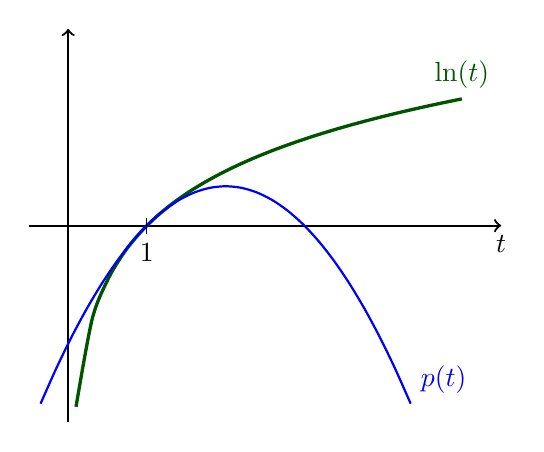
\begin{tikzpicture}
[
	closedpt/.style={circle,draw,fill,inner sep=0pt,minimum size=4pt},
	openpt/.style={circle,draw,inner sep=0pt,minimum size=4pt}
]

	% axes
	\draw[->,thick] (\xmin,0) -- (\xmax,0) node[below] {$t$};
	\draw[->,thick] (0,\ymin) -- (0,\ymax);

	% log graph
	\draw[very thick, green!33!black, domain=0.1:5, smooth] plot (\x,{ln \x}) node[above] {$\ln(t)$};

	% quadratic approximation at t=1
	\draw[thick, blue, domain=-0.35:4.35, smooth] plot (\x,{\x - 1 - (\x - 1)^2 / 2}) node[above right] {$p(t)$};

	\draw (1,0.1) -- (1,-0.1) node[below] {$1$};

\end{tikzpicture}
